\section{Protocolos Industriais}

Existem vários protocolos de comunicação industrial para diferentes aplicações. Dentre estes, podemos destacar 3 tipos de aplicação mais comuns:
\begin{enumerate}
    \item \label{it:0_1}Comunicação entre CLP e sensores e atuadores simples (nível 1 e nível 0).
    \item \label{it:1_2}Comunicação entre elementos do nível 1 (CLPs, CNCs, inversores, servomotores) e destes com supervisórios (nível 2).
    \item \label{it:2_3}Comunicação entre supervisórios e sistemas de gerência (nível 2 e nível 3).
\end{enumerate}

Redes de comunicação do tipo \ref{it:0_1} normalmente conectam um elevado número de dispositivos e requerem pequenos atrasos na comunicação, embora transmitam uma pequena quantidade de dados. Isto implica em um hardware simplificado, para permitir seu uso numa maior quantidade de dispositivos, e um protocolo determinístico, que permita controlar finamente o momento de aquisição de dados. Isto normalmente é conseguido usando uma camada física e de enlace própria da rede, tais como em redes Modbus RTU, HART, CAN, e AS-i.

Comunicações do tipo \ref{it:1_2} tem as mesmas características de requerer pequenos atrasos, mas acoplada a uma quantidade de dados bem maior, como por exemplo num robô industrial, em que se transmita a posição de cada um de seus eixos. Isto pode ser obtido com uma camada física e de enlace própria, como na Profibus DP, o que é custoso, tanto em termos de desenvolvimento quanto implementação, ou pela aplicação de uma camada ethernet como base da rede, como nas redes Modbus TCP, Profinet e EtherCAT.

Já comunicações do tipo \ref{it:2_3} são normalmente entre computadores e aí o uso delas sobre internet já é bem mais comum, como no caso de OPC-UA.

A tabela \ref{tab:protocolos} lista algumas características destes protocolos de redes industriais, para facilitar a comparação entre eles.

\begin{table}[h]
    \caption{Resumos de protocolos de redes industriais}\label{tab:protocolos}
    \begin{tabular}{l|cp{20mm}p{20mm}p{35mm}}
        \hline
        Protocolo & ano & velocidade & número de pontos & características\\
        \hline
        Modbus RTU & 1979 & $\sim$1~Mbps & 254 & Mestre escravo. Roda sobre RS432 ou RS485\\
        Modbus TCP & - & definido pela rede & ilimitado & Mestre escravo. Roda sobre TCP-IP\\
        HART & 1986 & & 15 & Definido como um sinal digital sobre um sinal 4-20 mA.\\
        CAN & 1987 & 512/128 kbps & indefinido & Provedor-. Acesso por CSMA-CD.\\
        Profibus DP & 1993 & 12~Mbps & 126 & \\
        Profinet &  & definido pela rede &  & \\
        AS-i & 1994 & & 62 & Comunicação e alimentação sobre apenas 2 fios.\\
        EtherCAT & 2003 & 100~Mbps & indefinido & Ethernet em anel para tempo real.\\
        OPC-UA & 2006 & & & \\
        \hline
    \end{tabular}
\end{table}

\subsection{Modbus}

O protocolo Modbus foi criado em 1979 e a princípio independe das camadas físicas e de enlace, definindo um pacote de transmissão da camada de transporte. Isto permite que se estabeleça uma rede Modbus com comunicação serial, sobre inernet, usando links de rádio ou até mesmo através de mensagens SMS.

Na prática, existem duas versões mais comuns de Modbus: Modbus RTU, que utiliza uma conexão serial como RS485, RS432 ou RS422, e Modbus TCP, que se conecta pelo protocolo TCP/IP.

A comunicação Modbus é feita através de pacotes, que se diferenciam entre a versão RTU e TCP, como pode ser visto nas tabelas \ref{tab:mbrtu} e \ref{tab:mbtcp}.

\begin{table}
    \centering
    \caption{Pacote Modbus RTU.}\label{tab:mbrtu}
    \begin{tabular}{r|c|c|c|c|c|c|}
        \cline{2-7}
        \textbf{Campo:} & início & endereço & função & dados & CRC & fim\\
        \cline{2-7}
        \textbf{\# bytes:} & 3,5 & 1 & 1 & $n$ & 1 & 3,5 \\
        \cline{2-7}
    \end{tabular}
\end{table}

No modbus RTU, os campos de início e fim na verdade indicam um tempo mínimo em que o canal deve ficar em silêncio. O endereço é o endereço de cada dispositivo, onde o mestre é o zero e podem ter até 254 escravos, dependendo das restrições da camada inferior. A função é o comando que está sendo dado pelo mestre ou respondido pelo escravo e a quantidade de dados depende justamente desta função. O CRC é \emph{Cyclical Redundancy Check}, um código de detecção de erros.

\begin{table}
    \centering
    \caption{Pacote Modbus TCP.}\label{tab:mbtcp}
    \begin{tabular}{r|c|c|c|c|c|c|}
        \cline{2-7}
        \textbf{Campo:} & ID de & ID de & tamanho & endereço & função & dados \\
         & transação & protocolo & pacote &  &  &  \\
        \cline{2-7}
        \textbf{\# bytes:} & 2 & 2 & 2 & 1 & 1 & $n$ \\
        \cline{2-7}
    \end{tabular}
\end{table}

No Modbus TCP, manda-se o pacote por TCP/IP, pela porta 502. O ID de transação define que pedaço da comunicação está sendo efetuado (0 para pedido de leitura, 1 para a resposta, etc.) e o ID de protocolo indica o protocolo que está sendo usado (valor é 2). O endereço é em geral ignorado, pois se usa diretamente o IP, e não se tem nem campos de início, fim ou CRC, que já são implementados na pilha TCP/IP.

O Modbus define 4 tipos de dados: \textbf{entradas discretas} ou \textbf{discrete inputs}, que são binários apenas de leitura; \textbf{bobinas} ou \textbf{coils}, binários de escrita e leitura; \textbf{registradores de entrada} ou \textbf{input registers}, que são \emph{words} de 16 bits de leitura e \textbf{holding registers}, de 16 bits e de leitura e escrita. Com base nestes tipos, as funções disponíveis mais comuns são:
\begin{description}
    \item[1] -- ler bobinas.
    \item[2] -- ler entradas discretas.
    \item[3] -- ler registradores holding.
    \item[4] -- ler registradores de entrada.
    \item[5] -- escrever numa única bobina.
    \item[6] -- escrever num único registrador holding.
    \item[15] -- escrever em múltiplas bobinas.
    \item[16] --  escrever em múltiplos registradores holding.
\end{description}

\subsection{HART}
HART é a sigla para \emph{Highway Addressable Remote Transducer}. Tem como principal característica ser um sinal digital enviado sobre um sinal analógico de 4 a \SI{20}{mA}. Tem seu uso como um protocolo ponto-a-ponto quando usado com esta característica, onde um tipo de sinal fica sendo transmitido de forma analógica enquanto outros, tais como outras medições, parâmetros do sensor ou sinais de calibração, são transmitidos de forma digital.

Um outro uso é efetivamente como rede, fazendo uma ligação em paralelo (\emph{multi-drop}) de vários dispositivos, alimentados através da corrente do loop, que neste caso fica fixa em \SI{4}{mA}. Dependendo da versão do protocolo, é possível conectar até 15 ou 64 dispositivos.

Como o HART manda o sinal digital sobre o de 4 a 20 mA, ele não pode definr 0 e 1 como uma grande diferença de tensão. Além disso, precisa de alguma forma enviar o dado serial sem o uso de um sinal de clock. Isto é conseguido usando a modulação FSK -- \emph{Frequency Shift Keying}, onde o bit 0 é transmitido como um sinal alternado de baixa amplitude (\SI{0,5}{mA}) com frequência \SI{2200}{Hz} e o 1 como um sinal da mesma amplitude na frequência \SI{1200}{Hz}.

É um protocolo mestre-escravo, tendo uma taxa de transmissão pequena, capaz de 2 mensagens por segundo. Pode também ser configurado peo mestre para usar um modo burst, onde o escravo fica mandando dados continuamente, a uma taxa de 3 mensagens por segundo.

Assim como no Modbus, usa um endereço para definir o escravo com que deseja se comunicar e um campo de comando, equivalente ao de função do Modbus. Tem alguns comandos HART que são aceitos por todo dispositivo HART, outro conjunto de \emph{best practices} que é implementado pela maioria dos dispositivos e pode ainda ter comandos específicos para determinado disppositivo.

\subsection{CAN}
Originalmente significava \emph{Car Area Network}, pois foi criado pela Bosch para fazer uma rede de sensores dentro de um carro. Atualmente tem seu uso em redes de sensores industriais, servindo de base para outros protocolos, tais como o DeviceNet. É um protocolo multi-mestre, com sistema de detecção de colisões na comunicação.

Este protocolo usa um par trançado como meio de comunicação, com os fios chamados de \emph{CAN Hi} e \emph{CAN Lo}, podendo ser conectado nos instrumentos (nós) de forma linear ou numa mistura de ligações lineares e em estrela (apenas no modo de tolerância a falhas, onde a velocidade fica limitada a \SI{128}{kbps}). Em ambos os casos o cabo tem um resistor de terminação conectando ambos os fios, o que faz com que a tensão diferencial entre eles se aproxime de \SI{0}{V} quando nenhum nó gera sinal.

O valor 0 no CAN (também chamado de dominante) é quando se aplica \SI{5}{V} ao \emph{CAN Hi} e \SI{0}{V} ao \emph{CAN Lo}, já o 1 (ou recessivo) é quando não se aplica sinal e o resisstor traz ambos os fios para próximo de \SI{2,5}{V}. Esta característica é usada na definição de prioridade de comunicação.

CAN é um protocolo produtor-consumidor, onde não se envia o endereço do nó mais sim um ID da própria mensagem, com 11 ou 29 bits, dependendo da versão do CAN. O nó que precisar daquela informação detecta pelo ID. Como o ID é o primeiro campo a ser transmitido, ele serve como definidor de prioridade da comunicação, pois quanto menor o ID, mais facilmente aquela mensagem consegue acesso ao barramento.

\textbf{Exemplo:} 2 nós querem acessar o barramento, sendo que um quer mandar uma mensagem de ID 1000
(0b01111101000) e outro com ID 500 (0b00111110111). Ambos os nós ficam lendo o barramento para detectar se está livre e começam a enviar a mensagem ao mesmo tempo. O primeiro bit é zero em ambos os casos e não há choque nenhum. O segundo bit é um 0 no que tem ID 500 e 1 no de ID 1000, como o 1 é recessivo, o barramento fica com valor 0. O nó que queria mandar a mensagem 1000 nota que o barramento está com um valor diferente edesiste de mandar, esperando outra oportunidade.

\begin{center}
\begin{tabular}{r|cccccc}
    \textbf{1000}       & \cellcolor{blue!25}0 & \cellcolor{red!25}1 & \multicolumn{4}{c}{\cellcolor{gray!25}desiste} \\
    \textbf{500}        & \cellcolor{blue!25}0 & \cellcolor{blue!25}0 & \cellcolor{red!25}1   & \cellcolor{red!25}1   & \cellcolor{red!25}1   & $\cdots$  \\
    \textbf{barramento} & \cellcolor{blue!25}0 & \cellcolor{blue!25}0 & \cellcolor{red!25}1   & \cellcolor{red!25}1   & \cellcolor{red!25}1   & $\cdots$ 
\end{tabular}
\end{center}

\subsection{DeviceNet}
O protocolo DeviceNet é um protocolo industrial implementado sobre o CAN. Ele aproveita o campo de ID do CAN para implementar um endereço de dispositivo com 6 bits, permitindo até 63 dispositivos.

O DeviceNet é feito para permitir retirada e colocação de dispositivos com a rede funcionando. Novs dispositivos começam com um escravo, com endereço 63 e depois são configurados com um novo endereço e com um de três possíveis modos de operação:
\begin{description}
    \item[Polled -- ]Neste modo os dispositivos continuam como escravos, apenas respondendo a pedidos de um mestre.
    \item[Cyclic -- ]Os dispositivos ficam enviando informação a intervalos definidos.
    \item[Change-of-State --] Enviam mensagens sempre que sua informação mudar. Eles também ficam enviando mensagens periodicamente mesmo que não mude de valor para que a rede saiba que ele continua funcionando.
\end{description}

\subsection{Profibus DP e PA}
Profibus foi criado na Alemanha em 1989, sendo adotado pela Siemens em vários equipamentos. Atualmente se usam 2 versões: Profibus DP (\emph{Decentralized Peripherals}) e Profibus PA (Process Automation). Ambos são basicamente o mesmo protocolo, só diferenciando na camada física, onde o PA é feito para ambientes com risco de explosão, o que limita sua velocidade. Isso faz com que uma rede Profibus DP possa ter dispositivos PA usando um simples conversor.

O Profibus é um protocolo onde os controladores são mestres e os dispositivos escravos, e a definição de qual mestre controla o barramento se dá por \emph{token passing}.

\subsection{Profinet}
Profinet é um protocolo industrial definido sobre uma rede ethernet, o que permite usar uma mesma rede para aplicações comuns e controle industrial. Dentro da especificação Profinet, 3 níveis são definidos: TCP/IP, que define o protocolo como uma aplicação em cima do protocolo TCP/IP, com tempos de resposta por volta de \SI{100}{ms}; RT (\emph{Real Time}), com tempos de ciclo menores que \SI{10}{ms} e IRT (\emph{Isochronous Real Time}), com tempos de ciclo menores que \SI{1}{ms} para aplicações de sistemas de posicionamento rápido e preciso, como em robôs industriais.

Os níveis RT e IRT requerem um hardware próprio para garantir a comunicação em tempo real, porém este hardware ainda deve ser compatível com aplicações ethernet comuns.

Apesar de serem redes diferentes, Profibus e Profinet são definidos pela mesma instituição e tem alguns elementos em comum, tais como a definição de funções e pontos de acesso dos dispositivos, o que torna a interligação de redes Profibus e Profinet simplificada. 

\subsection{AS-i}

A rede AS-i, \emph{Actuator Sensor Interface} foi desenvolvida para facilitar a conexão de dispositivos simples, tais como atuadores e sensores discretos. É uma rede com um único mestre e que usa um cabeamento próprio, incorporando alimentação e comunicação em apenas 2 fios.

O cabo mais comum de uma rede AS-i é um cabo amarelo com dois condutores paralelos, tal como na Figura \ref{fig:asi}. O cabo AS-i tem um perfil tal que impede a inversão da conexão, feita apenas pela prensagem do cabo num conector, que perfura o cabo com os dois terminais. Além disso, o material do cabo é \emph{cicatrizante}, isolando os furo caso se retire o conector.

\begin{figure}
    \centering
    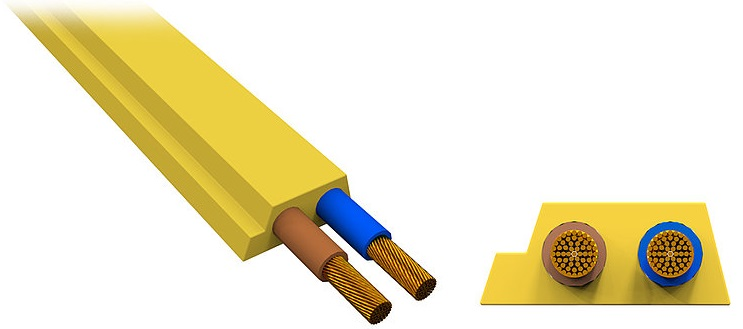
\includegraphics[width=\textwidth]{figuras/ASiCable}
    \caption{Cabo AS-i.}\label{fig:asi}
\end{figure}

Sobre este cabo vão a tensão de \SI{24}{V} para alimentar os escravos e o sinal de comunicação, que são pulsos de +2 e \SI{-2}{V} somados à tensão contínua. O pacote de comunicação AS-i permite endereçar até 62 escravos, enviando 5 bits de dados a cada escravo e recebendo 4 bits de dados. Ou seja, cada escravo pode ter 5 atuadores binários e 4 sensores binários. Uma rede completa com 62 escravos consegue se comunicar com todos 

\subsection{EtherCAT}

O protocolo EtherCAT, de \emph{Ethernet for Control Automation Technology}, é uma extensão do protocolo Ethernet que permite a comunicação em tempo real, com tempos de ciclo de menos que \SI{100}{\micro\second}. Para obter isso, a rede EtherCAT usa as mesmas camadas físicas e de enlace da ethernet, porém é conectada em anel e em vez de um pacote ethernet ser endereçado a apenas um dispositivo, na EtherCAT ele pode ter dados e comandos a vários, e eventualmente todos dispositivos da rede, que devem então receber o pacote, interpretá-lo, retirar a informação enviada a este dispositivo e anexar informações que ele deva enviar.

A necessidade de tratar e reenviar os pacotes a medida que vão chegando faz com que se necessite de um hardware específico em cada escravo ETherCAT, porém um servidor EtherCAT pode ser implementado como um aplicativo num computador sobre uma placa Ethernet padrão.

Atualmente existem vários dispositivos ETherCAT usando Ethernet 100BASE-TX, cuja taxa de \SI{100}{Mbps} \emph{full-duplex} é suficiente para todas aplicações. A princípio se pode ter EtherCAT sobre Gigabit Ethernet, mas ainda não se tem a necessidade para tal.

\subsection{OPC-UA}

OPC-UA (\emph{Open Platform Communications -- Unified Architecture}) é um protocolo de comunicação sobre internet que data de 2006. Ou seja, na pilha de protocolos TCP/IP ele conta como um aplicativo. Ele é definido numa licença \emph{open source} multiplataforma. É uma versão evoluída do protocolo OPC, que dependia de recursos exclusivos a plataformas Windows.

Há na verdade 2 protocolos definidos na especificação OPC-UA, um protocolo binário diretamente sobre TCP, mais difícil de ser implementado, porém com menor \emph{overhead}, e um sobre html, que requer mais recursos.

Dispositivos OPC-UA, ou nós, podem ser servidores ou clientes, e são definidos tais como objetos em linguagens de orientação a objetos, tendo atributos, que podem ser lidos, métodos, que podem ser executados e eventos que podem ser disparados. A especificação completa do OPC-UA é bastante extensa, ocupando 1250 páginas, divididas em 14 documentos. Normalmente a implementação é feita através de SDKs, em várias linguagens, tais como C, C++, Java ou Python.